\subsection{Semantics}
\label{sec:semantics}
%In this section, we describe generating process about the parser
%based on the ODL specification.
An in-memory representation is generated for each expression recursively,
which eventually builds into a complete parsing tree given an input XML.
Due to the fuzzy matching policy and the approximate spatial information
in the description, our parser can generate a number of candidate parse
trees.  The final results will be selected based on an optimization strategy.

\subsubsection{Input Data and Parse Result}
%ODL is a data description language for images.
Different from plain texts, OCR technique should be used in our procedure to
turn images into texts. Those semi-structured data contains both spatial information and content-based information so that we can reconstruct the physical
	layout of the images.
% The input of our generated parser is the XML.
In \figref{fig:data} we define the semi-structured data which is the set of all the text boxes at the word level as {\em input\_data}.

% which is the set of the text and coordinate pairs.
We also define the resulting parsing tree as a {\em parse\_tree},
which records the ODL expression and corresponding parsing result.
% \KZ{I'm confused by the above def. Is the data the XML? This should be made
% clear.}
\begin{figure}[ht!]
\centering
\begin{align*}
		   \text{text\_box} ::=~&\{c=\text{coor}, t=v\}\\
		   |~& \{\}\\
		   \text{parse\_tree} ::=~&((e,text\_box), [parse\_tree_1,...,parse\_tree_n])\\
		   |~& ()\\
\text{input\_data} ::=~&\{text\_box | ~~ \forall text\_box ~~in ~~XML\}\\
\end{align*}
\caption{input\_data and the parse\_tree}
\label{fig:data}
\end{figure}
\subsubsection{Correction Model}
\label{sec:corrmodel}
Besides the input data and the description in ODL, the fuzzy parser
also needs a correction model to correct the errors in the input data.
The generation of the correction model will be discussed in
\secref{sec:incremental}. Correction model $M$ is a set of correction
strategies $S$.
%\begin{equation}
%M=\{S |~~\forall generated ~~S\}
%\end{equation}
A simplified correction strategy is shown in \figref{fig:corrstrategy}.
Each correction strategy $S$ is a one-to-many mapping relationship between
the original substring in the OCR result and candidate result substrings
after correction. Each candidate is attached with a score,
which indicates that the probability of this candidate correction result is
the right answer for the original substring. For example, there's a 60\%
possibility that no correction is needed when given a letter ``b''.
In the fuzzy parser, for each text box in the input data, it will check
the correction model to find all the strategies that can be used
and generate new candidate text box content after correction.
If $m$ stands for the original substring and $A$ is the
set of the correct candidates and probabilities.
, a correction strategy $S$ can be represented as
\begin{equation}
S=\{(m, n, p)|~~\forall (n, p) \in A\}
\end{equation}
These candidates will be further filtered by using the scoring policies
discussed below.
\begin{figure}
\centering
\epsfig{file=figure/correctionStrategy.eps, width=0.3\columnwidth}
\caption{An Simplified Correction Strategy}
\label{fig:corrstrategy}
\end{figure}

\subsubsection{Scoring Policy}
\label{sec:score}
In the fuzzy parser, two scoring policies are designed
in order to solve fuzzy matching
problems in content-based data description and spatial information description respectively.

\paragraph{Scoring Policy for Data Description}
Due to the limitations of OCR techniques, data derived from images is not 100\%
correct. To tolerate the errors and noises in the OCR results, a scoring
policy is proposed to take consideration of the constraints and OCR results.

% For primitive expression, a error score is calculated based on the range,
% length and precision information.
% \KZ{What is base type expression? It wasn't
% mentioned before. And fix all the back quotes! If it's math expression or
% inline equation, use math mode $..$}
The calculation of error score $es(e, t)$ derived from the edit
distance. It uses an expression and a text box content in XML as inputs.
Specifically, we use the edit distance result as
the error score for the {\em constant}.
\begin{equation}
es(c, t) = ed(c, t)
\end{equation}
For the {\em name} of the integer and floating point type,
edit distances are calculated between the potential data and each number
which satisfies the range, length or precision information requirements.
The smallest edit distance is chosen as the error score.
If $Z$ is the set of all integers and $R'$ is the set of
all floating points that in length $l$ and precision $p$,
the error score is calculated as:
% \begin{multline}
\begin{equation}
es(x(int, a, b), t)=\min\{ed(i, t)| ~~\forall i \in Z, i \in \lbrack a, b \rbrack\}
\end{equation}
% \scalebox{0.8}{
% \parbox{1.2\textwidth}{
\begin{equation}
es(x(float, l, p, a, b), t)=\min\{ed(i, t)| ~~\forall i \in R', i \in \lbrack a, b \rbrack\}
\end{equation}
% }}
% \end{multline}
For example, if the expression is {\em constant} ``Vent. rate'' and
the value is ``Vcnt. rule,''
the error score will be the edit distance between them which is 2.
If the expression is {\em name} and {\em constraints} $x(int, 60, 100)$
and the value is ``53,'' the error score will be 1, since for all integers
between 60 and 100, one of the minimum edit distances with ``53'' is
the edit distance of ``63'' and ``53'', which is 1.

Using error score computation method, we can further compute $esm(e, t, M)$
which is the error score with the correction model. We first define $cor(t, S)$,
which takes a text box content $t$ and a correction strategy $S$ as inputs.
This function will give us a set of candidate corrected text box contents and
corresponding probabilities by replacing the substring of $t$ to new candidates
according to $S$. In $cor(t, S)$, $rep(t, m, n)=t'$ means that $t'$ is the
result of replacing all occurances of $m$ in the string $t$ with $n$.
\begin{equation}
cor(t, S)=\{(t',p)|~~\forall (m,n,p) \in S, rep(t,m,n)=t'\}
\end{equation}
Then the error score with correction model $esm(e, t, M)$ will
find the minimum product of the error score $es(e, t')$ and the probability $p$.
\begin{equation}
esm(e, t, M)=\min\{es(e, t')*p | ~~\forall S \in M, \forall (t', p) \in cor(t, S)\}
\end{equation}
% In the
% correction model, a substring of the OCR results is attached with the potentional
% right results and the probability for it being corrected as the new one.
% The generation of
% the correction model will be further explained in \secref{sec:correction}.
% \KZ{I'm not sure if I understood the following model correctly. C is not
% properly explained.}
% \begin{figure}
% \begin{equation}
%   \mbox{Correction Strategy:}~ C(oriStr)=newStr
% \end{equation}
% \begin{equation}
%   \mbox{Correction Model:}~ M = \{(C, Prob(C)) ~|~ \forall C\}
% \end{equation}
% \caption{Incremental Learning Model for Human Correction}
% \label{fig:corrModel}
% \end{figure}

% example
% \begin{algorithm}
% \caption{Error Score Computation Without Correction Model}
% \label{alg:errScore}
% \begin{algorithmic}
% \REQUIRE ~~\\
% The constant or name description $e$ and $data$.
% \ENSURE ~~\\
% The error score $errScore$
% \IF{$e$ is $c$}
% \STATE{$es$ = edit distance of $c$ and $data$}
% \ELSIF{$e$ is $x(int, min, max)$}
% 	\FOR{each integer $i$ between $min$ and $max$}
% 	\STATE{$es$ = the minimum edit distance between $i$ and $data$}
% 	\ENDFOR
% \ELSIF{$e$ is $x(float, l, p, min, max)$}
% 	\FOR{each floating-point $i$ with length l, precision p and between $min$ and $max$}
% 	\STATE{$es$ = the minimum edit distance between $i$ and $data$}
% 	\ENDFOR
% \ENDIF
% \end{algorithmic}
% \end{algorithm}

% \begin{algorithm}
% \caption{Error Score Computation With Correction Model}
% \label{alg:errScoreM}
% \begin{algorithmic}
% \REQUIRE ~~\\
% The constant or name description $e$, $data$ and correction model $m$
% \ENSURE ~~\\
% The error score with correction model $errScoreM$
% \FOR{each potentional correction result $dataCorrected$ of $data$ using $m$}
% \STATE{$errScoreM$ = the minimum product of $es$ between $e$ and $dataCorrected$ and
% the probability of $data$ being corrected as $dataCorrected$ }
% \ENDFOR
% \end{algorithmic}
% \end{algorithm}

The total score for the description is calculated by adding all the error scores
together. By adding all the error scores together, we can balance the tolerance for
errors in a sub expression and the overall sequence.
% \KZ{I think you can
% give a complete formula for the whole description.}
% example

\paragraph{Scoring Policy for Spatial Description}
In ODL, spatial description is used to describe the rough spatial
relationship based on human estimates. In order to minimize human efforts
in estimating the spatial distances, a spatial score $ss(coor, cc)$
is used, which measures the differences between the provided spatial
description and data.
% for handling such
% description fuzzily is used.
It takes the coordinates of the text box ($coor$) and the position of the current cursor ($cc$)
as inputs.
In the semantics, we record the position
of the parsing cursor, which is the current location of the parsing process.
For all potential input data, the spatial score is calculated according
to the distance between the data coordinates and the cursor.
% \begin{figure}[ht!]
% \begin{equation*}
\begin{equation}
	ss(cc, coor) = ||cc - coor||
\end{equation}
% \caption{Spatial Score Computation}
% \label{alg:ss}
% \end{equation*}
% \caption{Spatial Score Computation}
% \label{alg:ss}
% \end{figure}

\subsubsection{Evaluation Rules}

In those previous sections, we introduce some methods of processing the input data in order to tolerate some errors in the input data. In this section, we describe the evaluation rule for generating the parser.
The resulting parser is a list of all candidate parsing trees. Two scoring
policies are used to relieve the computational cost by filtering low probability results. Those specific rules for parsing are shown in Figure 14 in the form of inductive judgement forms. Those functions defined in Figure 13 would be used in the those inductive rules.
The {\em Cons} function is one of the key functions of parsing. It takes
the current position of the cursor $c$, a text box $tb$ and the expression $e$ as the input
and return true or false for whether the text box is a suitable candidate for the
expression. The function will evaluate the content of the text box based on
the scoring policy for data description and the spatial position
with the cursor according to the scoring policy for spatial description.
A threshold {\em t} is set for the sum of the two scores.
\begin{equation}
Cons(tb, c, e) =
\begin{cases}
\text{T}& \text{$esm(e, tb.t, M)+k*ss(c, tb.c) < t$}\\
\text{F}& \text{otherwise}
\end{cases}
\label{equ:constraint}
\end{equation}

The {\em Find} function is
designed for finding all potential results that satisfy the scoring policies.
The parsing process involves mapping the semi-structured data with the expression.
{\em Filter} is designed to filter the results based on the various constraints.
Due to
the spatial feature of the semi-structured data,
a variable named {\em c} is used
in the environment to record the position of the cursor.
In the judgement form that we designed to represent the parsing process, an ODL
expression, provided with the environment {\em E} and input data {\em D}, will be
evaluated into a list of parse trees and remaining data {\em D'}.
\[
  {\rm Judgment~ Form:}~~ E,D;e \Downarrow (D';parse\_tree)list
  \label{semantics:judegement}
\]
% where E is environment, D and D' are input\_data, C records the position of the cursor.

Evaluation rules \ref{rule:x}, \ref{rule:c1} and \ref{rule:c2} are used
for evaluating variable expression and constant expression respectively.
For each expression every given text box will be checked and will be
considered as a potential result if it satisfies the constraints.
For example, given {\em constant} ``Vent. rate'', current cursor at ``(132, 0)'' and some potential text boxes ``(c=$\langle$264,33, 336,45$\rangle$, t=``Vcnt. rule'')'' and ``(c=$\langle$264,51,439,64$\rangle$, t=``PR Interval'')'', the error score for the first text box is much lower compared to the second one. According to \ref{rule:c1}, the first text box will be considered as a potential result
for the expression and the second text box will not be a potential result, according to \ref{rule:c2}. For {\em name} and {\em constraints}, filtering based on the constraints will take place after generating all the results for the {\em name}.

Evaluation rule \ref{rule:coor}, \ref{rule:hskip} and \ref{rule:vskip}
are used for evaluating spatial operations. \ref{rule:coor} indicates that the data searching area
will be limited when providing coordinate information.
For example, in {\em constraints} expression ``e($\langle$0.1w,\_,0.5w,\_$\rangle$)'', ``w'' is short for the
width of the whole document, which is 1328 pixels and the length of the whole document is 1000 pixels in this case. All the data pairs outside of
the rectangle, for instance outside the upper left and bottom right corners of which are ``(132, 0)'' and ``(664, 1000)'', will not be considered.
\ref{rule:hskip} and \ref{rule:vskip}
indicates the remaining data after skipping.

For union, \ref{rule:union} indicates that each component
of the union description will be considered. For example, to parse the
{\em union} description (``month\_str'') used for the names of the months,
every possible month name will be tried and they will be filtered
by the constraints of the union expression and the context.
% The {\em union} description will be considered
% The
% {\em union} description will be considered {\em constant} ``Feb'' and generated corresponding candidate results together with the results when it is considered as the rest names.

{\em Struct} and {\em list} share
similar evaluation processes according to \ref{rule:struct} and \ref{rule:list}. These rules say
that data will be binding to them in sequence. For example, to parse the {\em struct} for ``triple'', the results for ``Vent. rate'' will be generated first, and then results for ``hskip $\backslash$s'' will be generated based on the remaining data after ``Vent. rate'' generation.

% \subsubsection*{Data Description Expression}
% The evaluation rule for variable description and constant description is described
% as \ref{rule:x1}, \ref{rule:x2}. The idea is that, based on the

% \subsection{Example}

\begin{figure}[ht!]
\tiny
\centering
% \begin{eqnarray*}
% \text{text~~box} ::=&&\{c=\text{coor}, t=v\}\\
% &&|\{\}\\
% \text{parse\_tree} ::=&&()\\
% &&|((e,text~~box), [parse\_tree_1,...,parse\_tree_n])\\
% \text{input~~data} ::=&& set ~~ of ~~ text~~boxs\\
% \end{eqnarray*}

\begin{align*}
% \centering
% \[
  Cons:text\_box~*&~coor*expression \rightarrow bool \\
% \]
% \[
  Find:input\_data~*&~coor*value \rightarrow input\_data \\
% \]
\end{align*}
\begin{align*}
% \centering
% \[
  Begin:&~input\_data \rightarrow coor \\
% \]
% \[
  End:&~input\_data \rightarrow coor \\
% \]
\end{align*}
%\vspace{-6 mm}
\[
  Filter:(input\_data*parse\_tree)list*expression \rightarrow (input\_data*parse\_tree)list 
\]
\[
  Hskip:input\_data*coor*(input\_data*parse\_tree)list \rightarrow input\_data 
\]
\[
  Vskip:input\_data*coor*(input\_data*parse\_tree)list \rightarrow input\_data 
\]

\caption{Functions in Semantics}\label{fig:funseman}
\end{figure}

\begin{figure}[ht!]
\tiny
% \[
%   {\rm Judgment~ Form:}~~ E,D;e \Downarrow (D';parse\_tree)list
%   \label{semantic:judegement} 
% \]
% where E is environment, D and D' are input\_data, C records the position of the cursor.
% \begin{minipage}[c]{0.45\textwidth}
\begin{gather*}
  \tag{\sc E-Empty}\label{rule:empty}
  \frac
  {}
  {E,\{\};x \Downarrow []}\\
  % \tag{\sc E-X1}\label{rule:x1}
  % \frac
  % {p \in D ~~ E(c)=coor ~~ Cons(p, coor, type)=true ~~ E,(D-p);x \Downarrow r}
  % {E,D;x \Downarrow (\{\};(x(type), p),[])::r}\\
  % \tag{\sc E-X2}\label{rule:x2}
  % \frac
  % {p \in D ~~ E(c)=coor ~~ Cons(p, coor, type)=false ~~ E,(D-p);x \Downarrow r}
  % {E,D;x \Downarrow (\{p\};(x(type), \{\}),[])::r}\\
  \tag{\sc E-C1}\label{rule:c1}
  \frac
  {p \in D ~~ E(c)=coor ~~ Cons(p, coor, const)=true ~~ E,(D-p);x \Downarrow r}
  {E,D;const \Downarrow ((D-p);(const, p),[])::r}\\
  \tag{\sc E-C2}\label{rule:c2}
  \frac
  {p \in D ~~ E(c)=coor ~~ Cons(p, coor, const)=false ~~ E,(D-p);x \Downarrow r}
  {E,D;const \Downarrow (D;(const, \{\}),[])::r}\\
  \tag{\sc E-X}\label{rule:x}
  \frac
  {p \in D ~~ E(c)=coor ~~ E,(D-p);x \Downarrow r}
  {E,D;x \Downarrow ((D-p);(x, p),[])::r}\\
  % \tag{\sc E-Name}\label{rule:name}
  % \frac
  % {E(x)=v ~~ E(c)=coor ~~ Find(D, c, v)=D'}
  % {E,D;*x \Downarrow \sum_{p_i \in D'}((D'-p_i);(*x, p_i),[])::[]}\\
  \tag{\sc E-Constraint}\label{rule:Constraint}
  \frac
  {E,D;e_0 \Downarrow r_0 ~~~~ \forall i: r_{i+1}=Filter(r_i, e_i)}
  {E,D;e_0(e_1, e_2, ..., e_n) \Downarrow r_{n+1}}\\
  \tag{\sc E-Coor}\label{rule:coor}
  \frac
  {Find(D, coor, nil)=D' ~~ E[c \mapsto Begin(D')],D';e \Downarrow (D'';t)list}
  {E,D;e(coor) \Downarrow (D-D'+D'';t)list}\\
  %\end{gather*}
  %\end{minipage}
  %\hfill \begin{minipage}[c]{0.45\textwidth}
  %\begin{gather*}
  % \frac
  % {E,D;e \downarrow r}
  % {E,D;e~~as~~x \Downarrow }\\
  \tag{\sc E-Hskip}\label{rule:hskip}
  \frac
  {E,D;e \Downarrow r ~~ E(c)=coor ~~ Hskip(D, coor, r)=D'}
  {E,D;hskip~~e \Downarrow (D';[])::[]}\\
  \tag{\sc E-Vskip}\label{rule:vskip}
  \frac
  {E,D;e \Downarrow r ~~ E(c)=coor ~~ Vskip(D, coor, r)=D'}
  {E,D;vskip~~e \Downarrow (D';[])::[]}\\
  \tag{\sc E-Union}\label{rule:union}
  \frac
  {E,D;e_1 \Downarrow r_1 ~~ E,D;\{e_2|..|e_n\} \Downarrow r_2}
  {E,D;\{e_1|e_2|...|e_n\} \Downarrow r_1+r_2}\\
  \tag{\sc E-Sturct}\label{rule:struct}
  \frac
  {E,D;e_1 \Downarrow (E',D';parse\_tree)list~~~~  \forall i:  E'_i[c \mapsto End(D-D_i')],D_i';\{e_2,...,e_n\} \Downarrow r_i}
  {E,D;\{e_1,e_2,...e_n\} \Downarrow \sum_{i=1}^{m} (D';parse\_tree)list*r_i}\\
  \tag{\sc E-List}\label{rule:list}
  \frac
  {E,D;head ~~e~~list \Downarrow (E',D';parse\_tree)list ~~~~ \forall i:  E'_i[c \mapsto End(D-D_i')],D_i';tail~~e~~list \Downarrow r_i}
  {E,D;e~~list \Downarrow \sum_{i=1}^{m} (D';parse\_tree)list*r_i}\\
  % \tag{\sc E-List}\label{rule:list}
  % \frac
  % {E,D;e \Downarrow (E',D';parse\_tree)list ~~~~ }
  % {E,D;e ~~ list \Downarrow }\\
\end{gather*}
%\end{minipage}
\caption{Semantics}\label{fig:semantics}
\end{figure}


% Describe the process of parser generation.
% \begin{enumerate}
% \item Using inference rules;
% \item How to use the spatial information we have;
% \item How to design the scoring policy to handle the noises and errors.
% \end{enumerate}

% \begin{figure}
% % \centering
% \begin{eqnarray*}
% \text{pair} ::=&&\{c=\text{coor}, t=v\}\\
% &&|\{\}\\
% \text{tree} ::=&&[]\\
% &&|((e,pair), [t_1,...,t_n])\\
% % \text{data} ::=&&pair ~~ list\\
% % \text{report} ::=&&pair\\
% % &&|NF\\
% % &&|pair ~~ list\\
% % \text{map} ::=&&\{e=v, r=report\}\\
% % \text{maps} ::=&&map ~~ list\\
% % \text{result} ::=&&\{\{v_1,pair_1\}, ..., \{v_n,pair_n\}\}\\
% \end{eqnarray*}
% \caption{Data}\label{fig:data}
% \end{figure}

% \begin{figure}
% % \centering
% \begin{eqnarray*}
% % \text{parse}(e, data) ::=&& \text{parse}(v, date)\\
% \text{score}(maps):&& maps->float\\
% % \text{opt}(maps ~~ list):&& maps ~~ list->map~~list\\
% \text{opt}(maps ~~ list):
% &&if ~~ score(head~~(maps~~list))>score(opt(tail~~(maps~~list)))\\
% &&then ~~ head~~(maps~~list)\\
% &&else ~~ opt(tail~~(maps~~list))\\
% \text{limit}(coor, data):
% &&if ~~ (head ~~ data).c \in coor\\
% &&then ~~ (head ~~ data)::limit(coor, tail~~data)\\
% &&else ~~ limit(coor, tail~~data)\\
% \text{used\_data}(maps):
% &&if ~~ (head~~maps).r != NF\\
% &&then ~~ (head~~maps).r::used(tail~~maps)\\
% &&else ~~ used\_data(tail~~maps)\\
% \text{remain\_data}(maps, data):
% &&data-used\_data(maps)\\
% \text{parse}(x, pair):
% &&let ~~ map ~~ = \{e=x, r=pair\}~~in\\
% &&if~~score(map)>threshold\\
% &&then~~map::[]\\
% &&else~~\{e=x, r=NF\}::[]\\
% \text{parse}(x, data):
% &&let ~~ mapslist ~~ = parse(x, head~~data)::parse(x, tail~~data)::[]~~in\\
% &&opt~~(mapslist)\\
% \text{parse}(e=\{e_1 | e_2 | ... | e_n\}, data):
% &&let ~~ mapslist ~~ = parse(first~~e, data)::parse(rest~~e, data)::[]~~in\\
% &&opt~~(mapslist)\\
% % doubt
% \text{parse}(e=\{l_1 = e_1, ..., l_n = e_n\}, data):
% &&let ~~ maps = parse(head~~e, data)~~in\\
% &&maps::parse(tail~~e, remain\_data(maps, data))\\
% % &&if ~~ type((head ~~ e)) ~~ is ~~ record\\
% % &&then ~~ combine(parse(head ~~ e, data), parse(tail~~e, remain_data))\\
% % &&else ~~
% \text{parse}(e=e_0{_{(coor)}}, data):
% &&let ~~d_{limit} = limit(coor, data)\\
% &&parse(e_0, d_{limit})\\
% \text{parse}(e=e_0 ~~ list, data):
% &&let ~~ maps = parse(head~~e, data)~~in\\
% &&maps::parse(tail~~e, remain\_data(maps, data))\\
% \text{parse}(e.l, data):
% &&let ~~ e_1 = e.l ~~in\\
% &&parse(e_1, data)\\
% \text{parse}(e=hskip ~~ e_1, data):
% &&let ~~ pairlist = \\
% &&if ~~ e_1>0\\
% &&then ~~ (head~~data)::parse(e=hskip~~(e_1-(head~~data).coor.length), tail~~data)\\
% &&else []\\
% &&in ~~ \{e=hskip~~e_1, r=pairlist\}::[]\\
% % \text{parse}(e=vskip ~~ e_1, data):
% % &&let ~~ pairlist = \\
% % &&if ~~ e_1>0\\
% % &&then ~~ \\
% % &&let ~~ remain = \\
% % &&if ~~
% % (head~~data)::parse()
% % &&\text{parse}(e_{(coor)}, data)=\\
% % &&~~d_{limit} = \{p | p \in data.i, ~~ p.coor \in coor \}\\
% % &&~~\text{parse}(e, d_{limit})\\
% % &&\text{parse}(v, line)=\\
% % &&~~results ~~ = cons[result] ~~ nil[result] ~~ \text{parse}(v, head[pair] ~~ line)\\
% % &&~~results ~~ = cons[result] ~~ results ~~ \text{parse}(v, tail[pair] ~~ line)\\
% % &&~~return ~~ opt(results)\\
% % &&~~for ~~ pair ~~ in ~~ line:\\
% % &&~~~~results ~~ add ~~ (v, pair)\\
% % &&~~return ~~ opt(results)\\
% % &&\text{parse}(v, data)=\\
% % &&~~for ~~ line ~~ in ~~ data:\\
% % &&~~~~results ~~ add ~~ \text{parse}(v, line)\\
% % &&~~return ~~ opt(results)\\
% \end{eqnarray*}
% \caption{Semantic}\label{fig:semantic}
% \end{figure}

% \begin{figure}[ht!]
% \centering
% \begin{equation}
%  generate:expresion*data \rightarrow \{parse\_tree, remain\_input\} ~~ list
% \end{equation}
% \begin{equation}
%   score:parse\_tree \rightarrow float
% \end{equation}
% \begin{eqnarray*}
%   \lefteqn{generate(x, pair::data)=}\\
%   &&let \\
%   &&~~ tree = leafnode(\{x, pair\})\\
%   &&in\\
%   &&~~ \{tree, data\}::generate(x, data)\\
%   \lefteqn{generate(e=\{e_1 | e_2 | ... | e_n\}, pair::data)=}\\
%   &&append ( generate(e_1, pair::data) , generate(\{e_2|...|e_n\}, pair::data))\\
%   \lefteqn{generate(e=\{l_1 = e_1, ..., l_n = e_n\}, pair::data)=}\\
%   &&let\\
%   &&~~ combine(tree_1, \{tree_2, ri\}::remainlist) = \\
%   &&~~~~ \{(tree_1;tree_2), ri\}::combine(tree_1, remainlist)\\
%   &&~~ help(\{pt, ri\}::results) = \\
%   &&~~~~ append (combine(pt, (generate(tail ~~ e, ri))), help(results))\\
%   &&in\\
%   &&~~ help(generate(head ~~ e, pair::data))\\
%   \lefteqn{generate(e = e_0 ~~ list, pair::data)=}\\
%   &&let\\
%   &&~~ combine(tree_1, \{tree_2, ri\}::remainlist) = \\
%   &&~~~~ \{(tree_1;tree_2), ri\}::combine(tree_1, remainlist)\\
%   &&~~ help(\{pt, ri\}::results) = \\
%   &&~~~~ append (combine(pt, (generate(tail ~~ e, ri))), help(results))\\
%   &&in\\
%   &&~~ help(generate(head ~~ e, pair::data))\\
%   \lefteqn{generate(e=e_0{_{(coor)}}, pair::data)=}\\
%   &&let\\
%   &&~~ limit(coor, pair::data) = \\
%   &&~~~~ if ~~ pair.c \in coor\\
%   &&~~~~ then ~~ \{pair::limit(coor, data).1, limit(coor, data).2\}\\
%   &&~~~~ else ~~ if ~~ pair.c ~~ after ~~ coor\\
%   &&~~~~ then ~~ \{limit(coor, data).1, pair::limit(coor, data).2\}\\
%   &&~~~~ else ~~ \{limit(coor, data).1, limit(coor, data).2\}\\
%   &&~~ data_{limit} = limit(coor, pair::data).1\\
%   &&~~ data_{remain} = limit(coor, pair::data).2\\
%   &&~~ combine(data_{re}, \{tree, ri\}::results) = \\
%   &&~~~~ \{tree, data_{re}::ri\}::combine(data_{re}, results) \\
%   &&in\\
%   &&~~ combine(data_{remain}, generate(e_0, data_{limit}))\\
%   \lefteqn{generate(e.l, data)=}\\
%   &&let\\
%   &&~~ e_1 = e.l\\
%   &&in\\
%   &&~~ generate(e_1, data)\\
%   \lefteqn{generate(e=(hskip e_0), pair::data)=}\\
%   &&if ~~ e_0 > 0 ~~ and ~~ pair != newline\\
%   &&then ~~ combine(leafnode{pair}, generate(hskip (e_0-pair.length), data))\\
%   &&else ~~ []\\
%   \lefteqn{generate(e=(vskip e_0), data)=}\\
%   &&if ~~ e_0 > 0 ~~ and ~~ pair == newline \\
%   &&then ~~ combine(leafnode{pair}, generate(vskip (e_0-pair.height), data))\\
%   &&else ~~ if ~~ pair != newline\\
%   &&then ~~ combine(leafnode{pair}, generate(vskip e_0, data))\\
%   &&else ~~ []\\
% \end{eqnarray*}
% \caption{Semantic}\label{fig:semantic}
% \end{figure}
